
\section{Ejercicio 2.}

La red de este ejercicio trata de una comunidad de delfines de Doubtful Sound, Nueva Zelanda. La comunidad, que se constituye de 62 ejemplares identificados por una marca en la aleta dorsal, fue fotografiada entre 1995 y 2001. Los datos consisten en un número identificador para cada delfín, su nombre, su género (para 4 ejemplares no está especificado) y la información sobre entre qué pares de ejemplares se forma un link. La red es no dirigida, y contiene un total de 159 links, donde se establece que existe un link entre aquellos individuos que fueron vistos juntos de forma más frecuente que la esperada aleatoriamente, es decir, por un criterio de ``compañía preferida".\footnote{D. Lusseau, The emergent properties of a dolphin social network, Proc. R. Soc. London B (suppl.) 270, S186-S188 (2003).}
\par El ejercicio se dividió en tres partes: en la parte (a), exploramos diferentes layouts para la visualización del grafo; en la parte (b), nos preguntamos si la red es homofílica, es decir, si un delfín tiende a formar enlaces con aquellos ejemplares del mismo género; y en la parte (c), proponemos un método para descomponer la red en dos comunas quitando la menor cantidad de nodos posibles.

\subsection{Parte a.}

\begin{figure}
\centering
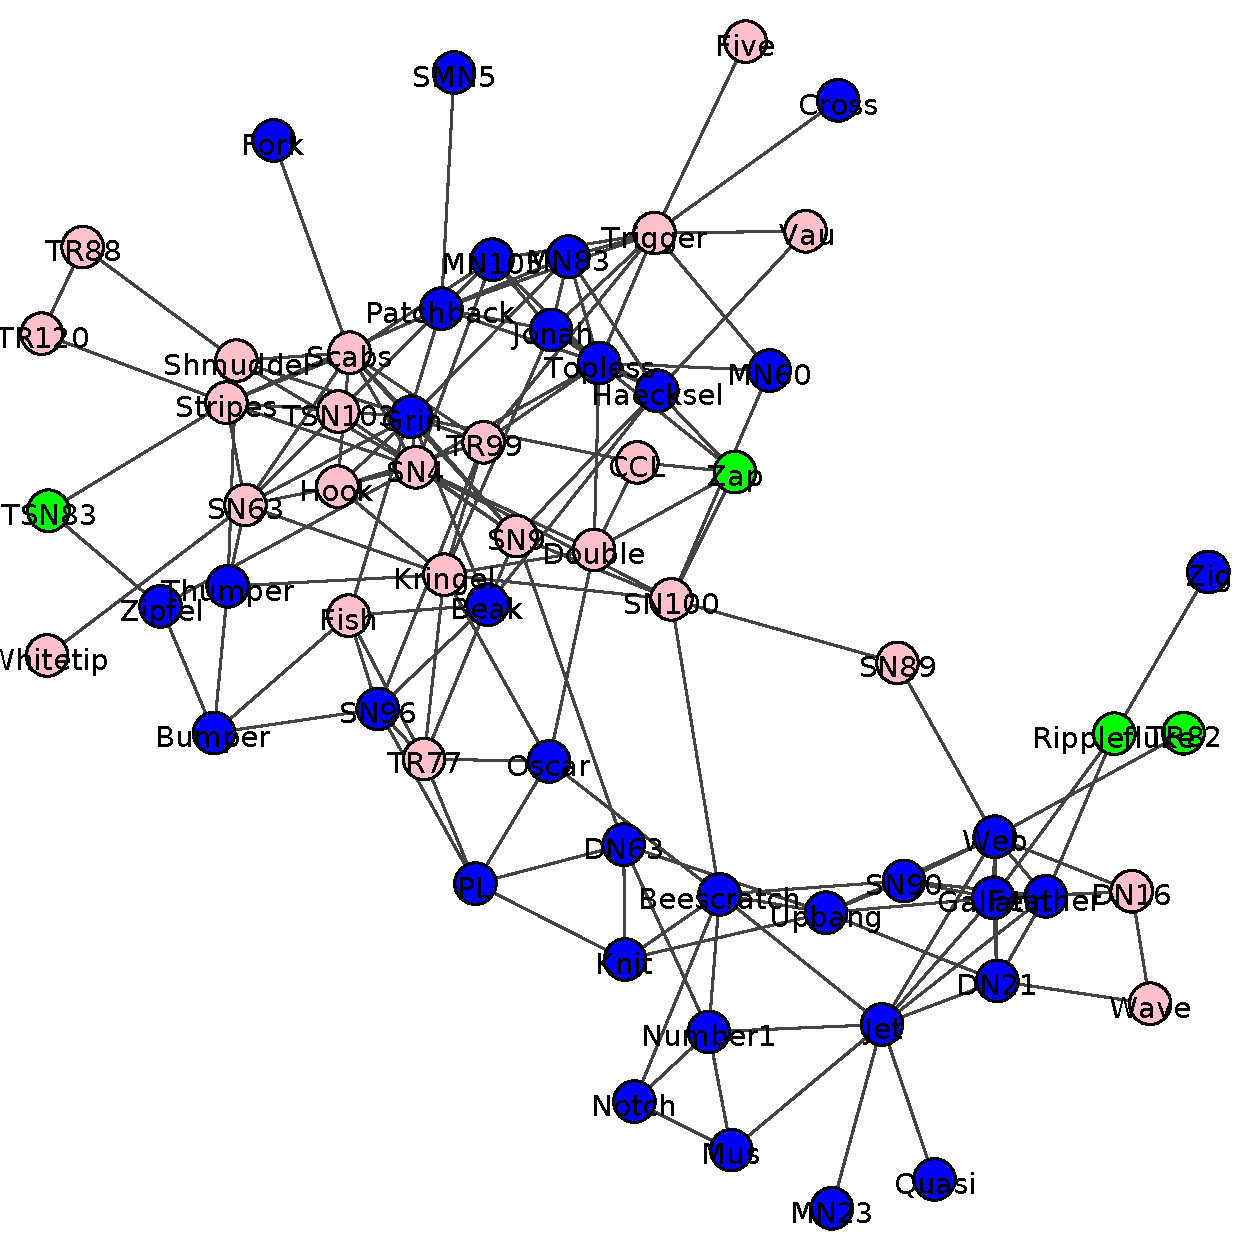
\includegraphics[scale = 0.50]{figuras/FrutRein-eps-converted-to.pdf}
\caption{Fruchterman - Reingold layout. Los colores de los nodos se refieren al sexo del delfín: azul, macho; rosa, hembra; verde, sexo no indicado en el dataset. A partir de este layout se puede intuir la existencia de dos comunas de delfines ligadas por pocos nodos.}
\label{fig:Layout_delfines}
\end{figure}

\par En esta primera parte del ejercicio, exploramos diferentes layouts para visualizar la red delfines.
En la figura \ref{fig:Layout_delfines} observamos el resultado de graficar
el grafo con el Fruchterman - Reingold layout. El algoritmo para realizar este layout se basa en asignarles fuerzas de interacción ficticias a los nodos. Típicamente se basa en que los nodos ligados tengan una fuerza de atracción análoga a la fuerza de un resorte, sumado a una fuerza de repulsión entre todos los nodos, análoga a la interacción coulombiana entre partículas cargadas idénticamente.\footnote{https://en.wikipedia.org/wiki/Graph\_drawing}
Este estilo de layout nos permitió visualizar la existencia de dos comunas de delfines, ligadas a través de unos pocos nodos.
\par Otros layouts que nos aportan la misma intuición son el DrL layout y el Kamada Kawai (fig. \ref{fig:Layouts_alternativos}), que también están basados en la asignación de fuerzas ficticias. Preferimos el Fruchterman - Reingold layout, ya que los nodos aparecen mejor distribuidos, y permite una mejor visualización de la red.
A modo de ejemplo, en la figura \ref{fig:Layouts_malos} incluímos otros layouts: Random, que sitúa los nodos en forma aleatoria, y Multidimensional Scaling, que se basa en una proyección matricial a un espacio de baja dimensionalidad, que no nos aportaron una buena visualización.

\begin{figure}
\centering
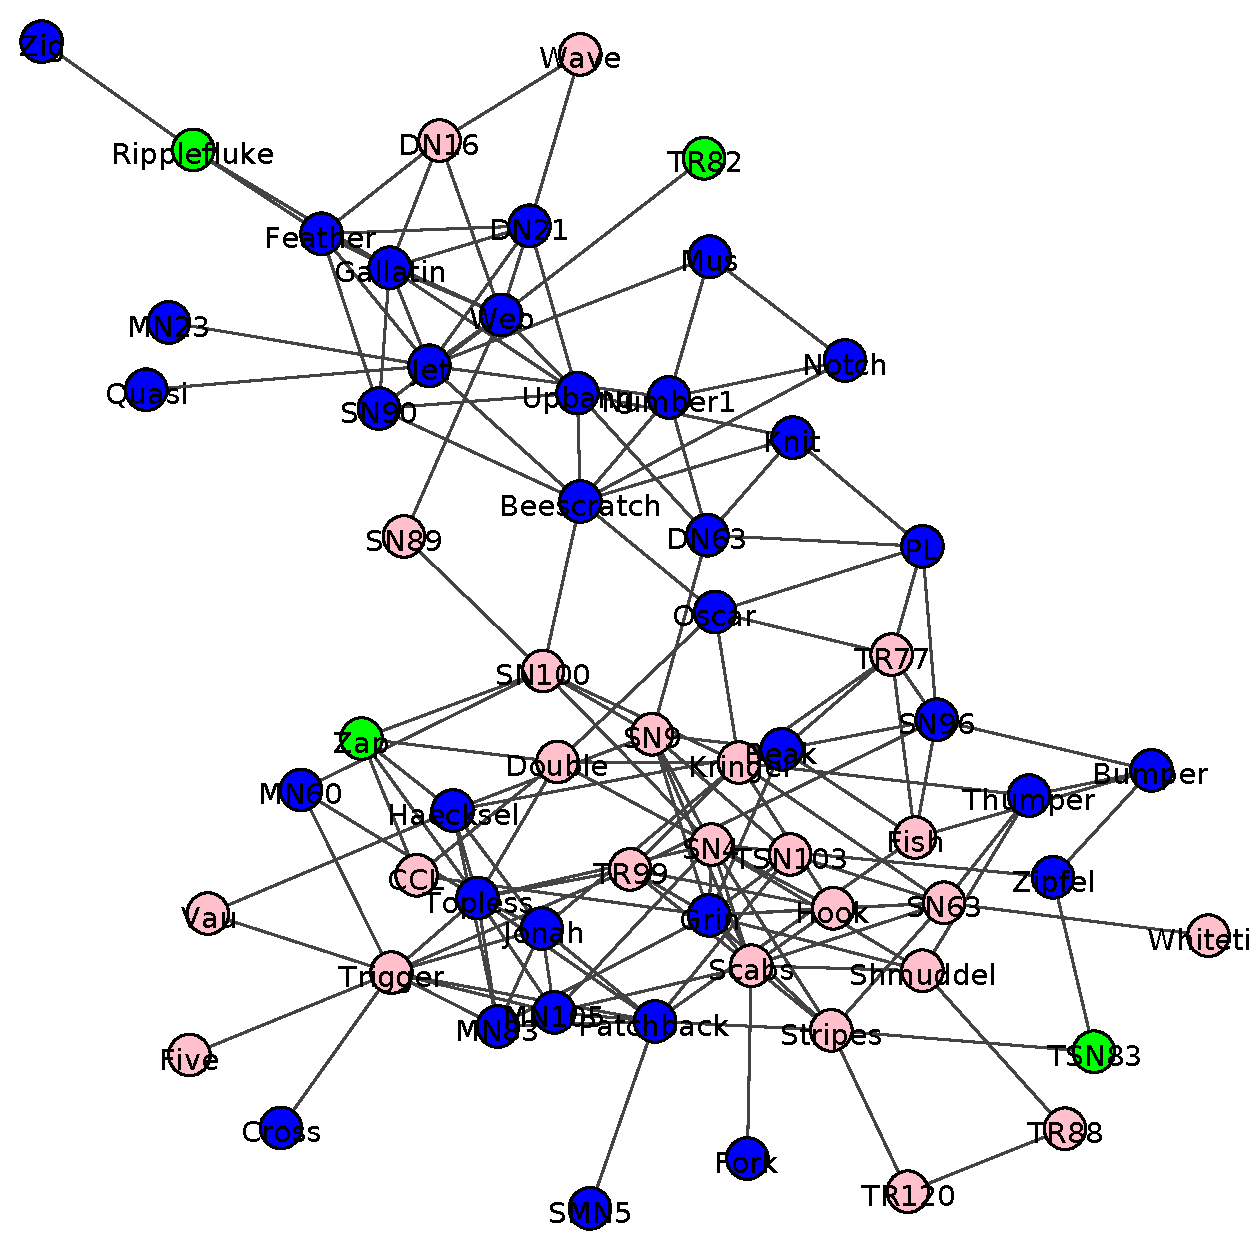
\includegraphics[scale = 0.25]{figuras/KamKaw-eps-converted-to.pdf}
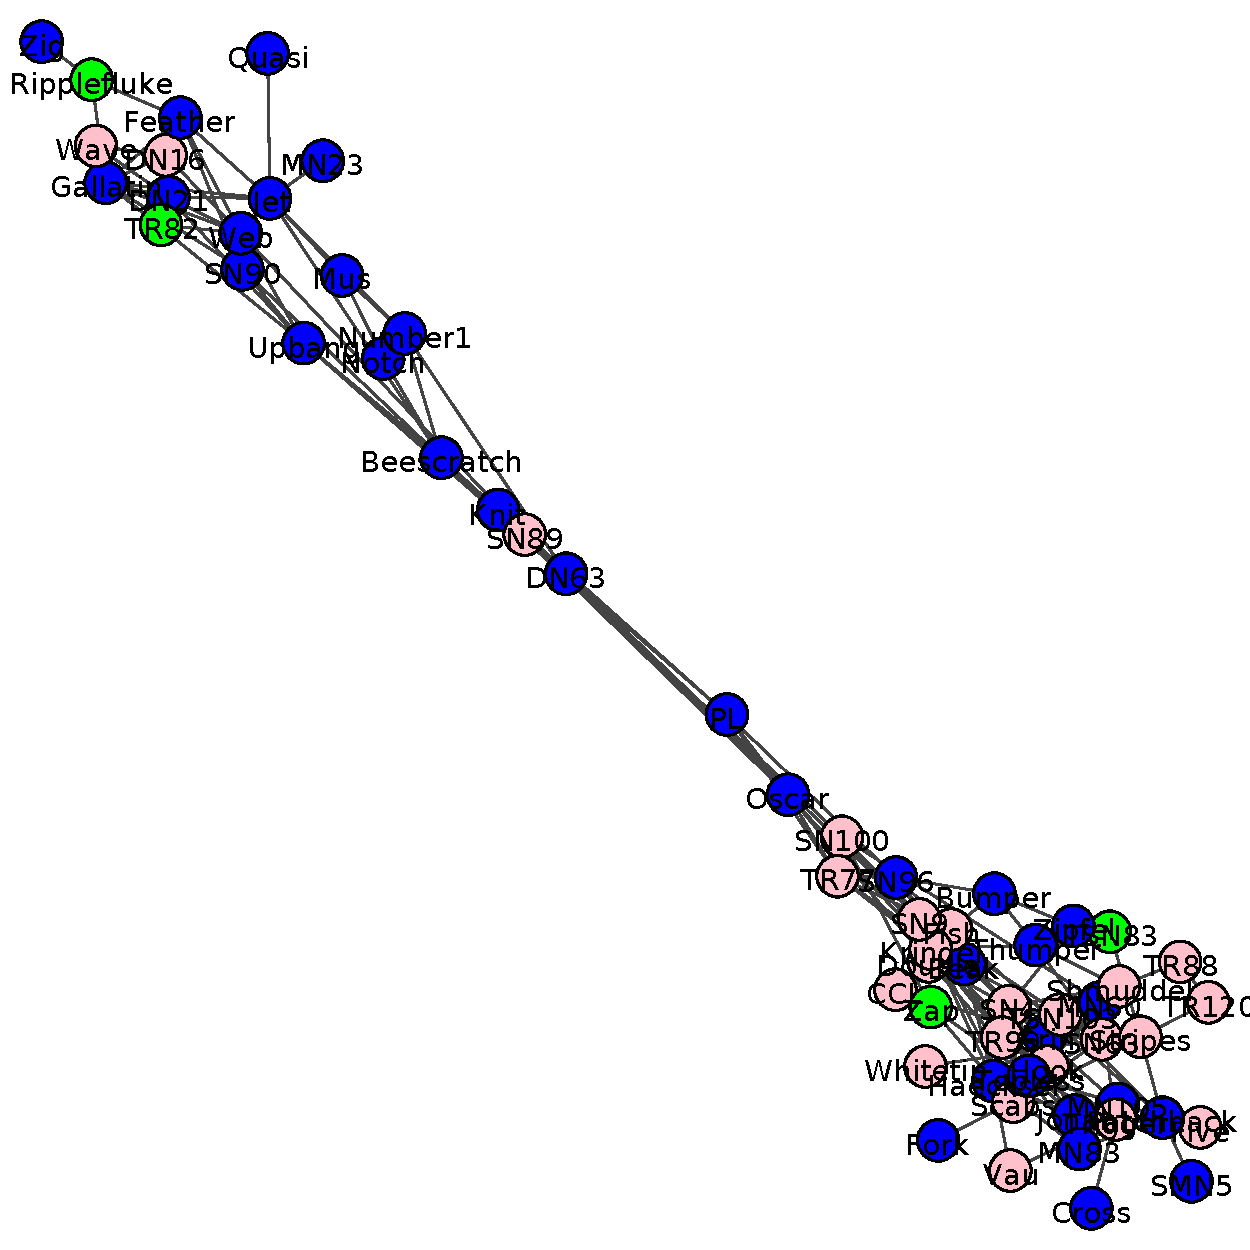
\includegraphics[scale = 0.25]{figuras/Drl-eps-converted-to.pdf}
\caption{Layouts alternativos: Kamada Kawai izquierda, DrL derecha. Estos también dan la información de una red con dos comunas de tamaño comparable.}
\label{fig:Layouts_alternativos}
\end{figure}

\begin{figure}
\centering
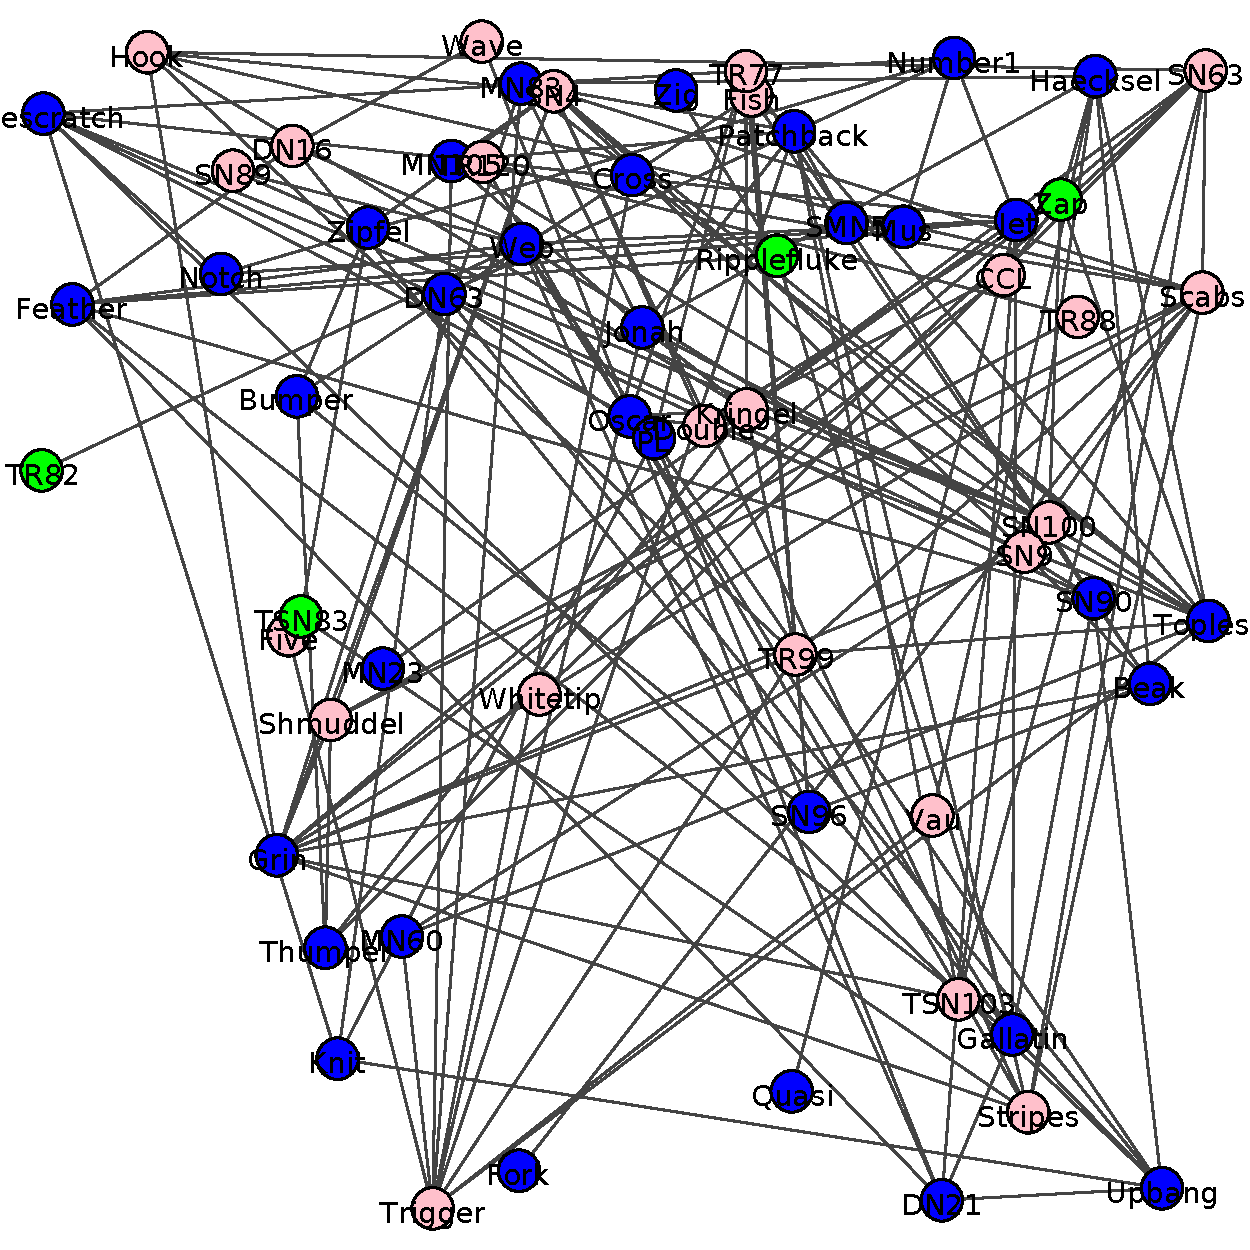
\includegraphics[scale = 0.25]{figuras/Random-eps-converted-to.pdf}
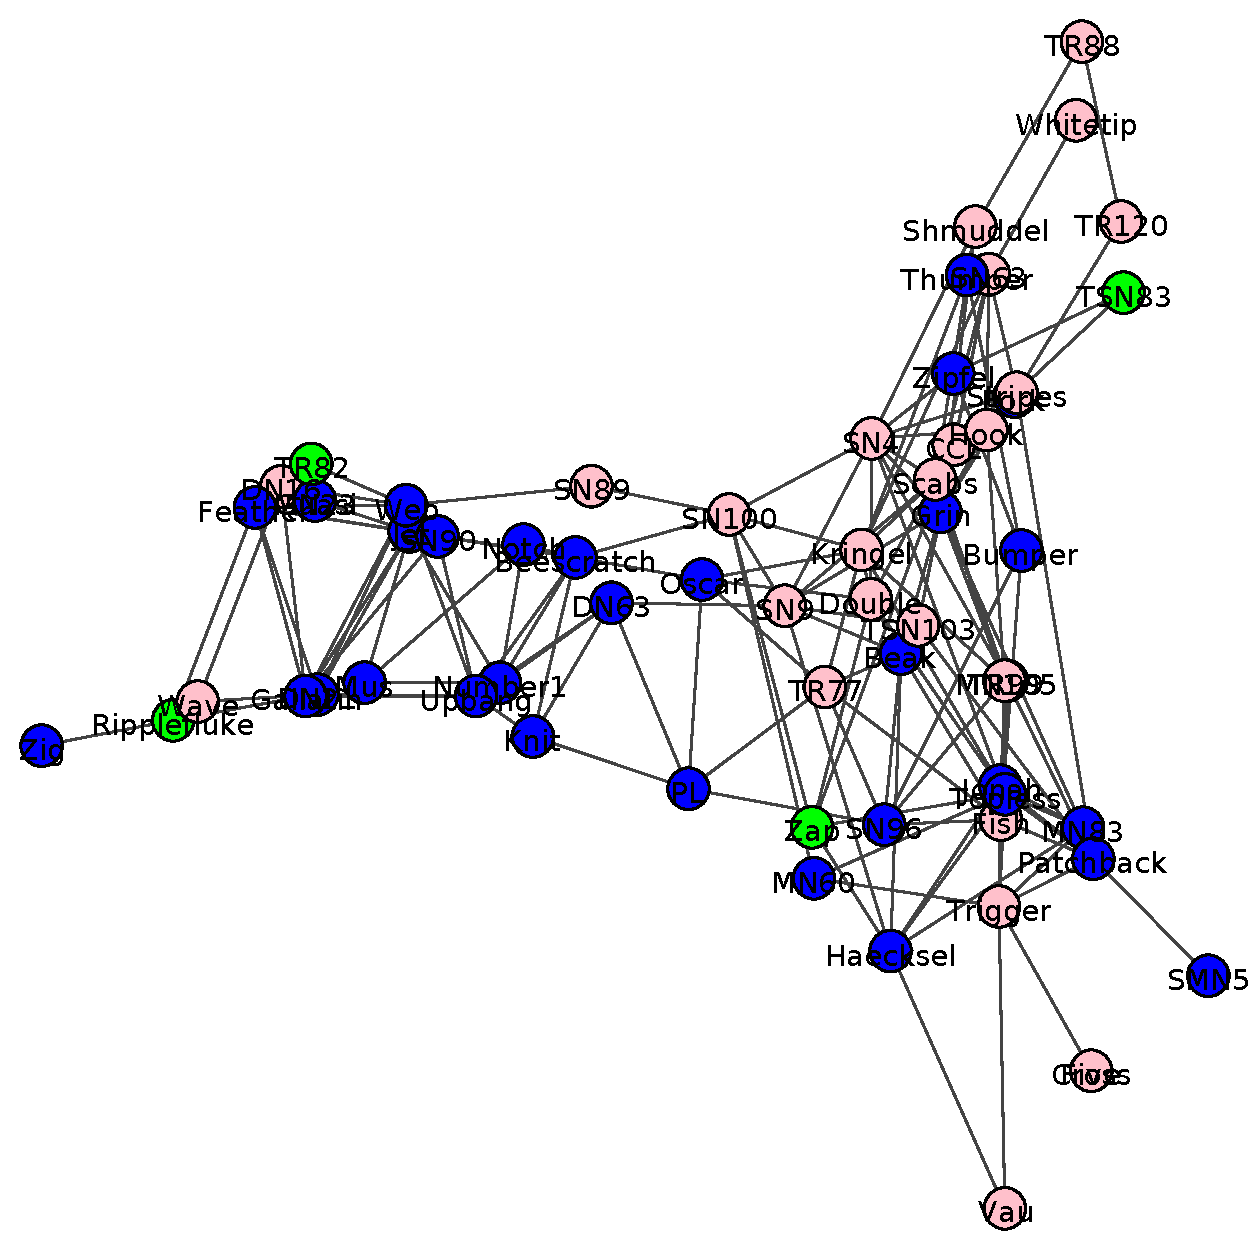
\includegraphics[scale = 0.25]{figuras/Multi-eps-converted-to.pdf}
\caption{Layouts que no permiten una buena visualización del problema: Random izquierda, Multidimensional Scaling derecha.}
\label{fig:Layouts_malos}
\end{figure}


\subsection{Parte b.}

\par En esta parte nos propusimos estudiar si la red es de carácter homofílica, es decir, si un dado nodo tiende a ligarse con nodos que comparten una característica con él, como es en este caso el género de los delfines. Para ello consideremos la hipótesis nula, es decir, que la asignación de género a un dado nodo es totalmente independiente de la topología de la red, y comparamos con lo presente en el dataset.
\par La metodología empleada fue la siguiente: sorteamos el género de los delfines manteniendo inalterable la topología de la red y manteniendo constante la cantidad de delfines machos, hembras, y género no específicado de la red original. Generamos $10^{6}$ realizaciones distintas, y para cada caso calculamos la cantidad de links entre delfines de distinto género (sin tomar en cuenta los links entre pares de nodos que incluya un género indefinido). El resultado es la distribución de la figura \ref{fig:Histograma}.
De dicha distribución obtuvimos un valor medio de links entre géneros $<m> = 68 \pm 7$. Dado que el número de links totales ($N'$) es $N' = 159$, la fracción de links entre géneros es:
\begin{align*}
	(\frac{<m>}{N'})_{hip.nula} & = 0.43 \pm 0.04
\end{align*}
En la figura \ref{fig:Histograma}, incluímos la cantidad de links entre géneros de la red real, que en principio se observa mucho menor que la media de la distribución.

\begin{figure}
\centering
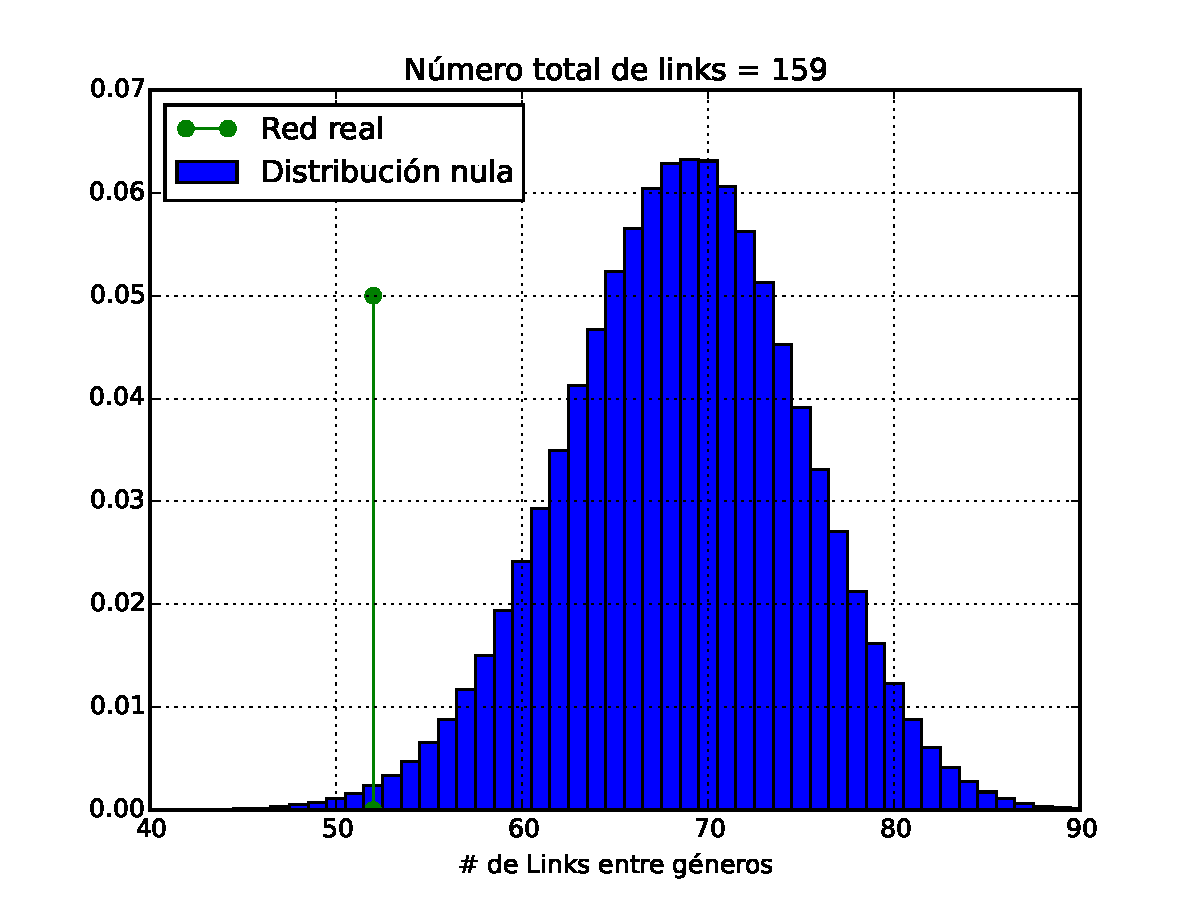
\includegraphics[scale = 0.70]{figuras/Histograma-eps-converted-to.pdf}
\caption{Histograma de links entre géneros sorteando sobre la topología de la red. En verde, cantidad de links entre géneros de la red actual (la altura de la barra no representa nada especial, es solo indicativa).}
\label{fig:Histograma}
\end{figure}

\par Por otro lado podemos estimar analíticamente la fracción de links entre géneros que habría para una red aleatoria. Si tomamos que la probabilidad de escoger un link entre un macho y una hembra es $2 \rho_{M} \rho_{F}$, donde $\rho$ son las densidades de cada género en la red real ($M$ para macho, $F$ para hembra), entonces la probabilidad de tomar $m$ links de esta característica es:
\begin{equation}
	P(m) = {N' \choose m} (2 \rho_{M} \rho_{F})^{m} (1 - 2 \rho_{M} \rho_{F})^{N' - m}
\end{equation}
donde $N' = N(N-1)/2$, que es el número total de links que se pueden formar en una red de $N$ nodos. Con esta distribución, el valor medio de links y la desviación standard resultan:
\begin{align*}
	<m> & = 2 N' \rho_{M} \rho_{F} \\
	std(m) & = (2 N' \rho_{M} \rho_{F} (1 - 2 \rho_{M} \rho_{F}))^{1/2}\\
\end{align*}
Por lo tanto, la fracción de links ($<m>/N'$) para las densidades de género actuales, estimado mediante la ecuación anterior, resulta:
\begin{align*}
	(\frac{<m>}{N'}){estimado} & = 0.43 \pm 0.01
\end{align*}
Observamos que el valor estimado y el obtenido sorteando al azar el género de los delfines coindicen.
\par Como puede deducirse de la figura \ref{fig:Histograma}, la probabilidad de que se obtengan la cantidad de links entre géneros de la red actual dada la hipótesis nula es menor a $0.005$, por lo que descartamos la hipótesis nula, y concluimos que la red es homofílica: la cantidad de links entre géneros es mucho menor que el valor esperado si la distribución de géneros fuera aleatoria, lo que implica que hay más cantidad de enlaces entre delfines del mismo sexo que entre ejemplares de distinto género, y además la probabilidad que el valor actual se dé por simple aleatoriedad es muy baja.

\subsection{Parte c.}

\par Como último punto, proponemos un método para dividir la red en dos componentes de tamaño comparable. Debido a que suponemos que la red se constituye principalmente de dos comunas ligadas por pocos nodos, consideramos que el cálculo del betweenness no dará información sobre dichos nodos. El betweenness tiene en cuenta la cantidad de caminos cortos que pasan por un dado nodo. Su remoción implicaría un aumento en la distancia entre nodos. Formalmente, el betweenness de un nodo se calcula como:
\begin{equation}
	Bet(i) = \sum_{j,k} \frac{b_{jik}}{b_{jk}}
\end{equation}
donde $b_{jk}$ es el número de caminos cortos que van desde $j$ hasta $k$, y $b_{jik}$ es el número de caminos cortos que van desde $j$ hasta $k$, que pasan por $i$.
\par Removiendo los nodos con mayor betweenness, basta remover 4 nodos para descomponer la red en dos conjuntos no conexos, como puede observarse en la figura \ref{fig:Betweenness}. Si lo comparamos con el caso de remover nodos al azar sin más criterio, es muy díficil obtener este resultado. En la figura \ref{fig:Comparacion}, mostramos el tamaño del componente conectado más grande del sistema a medida que removemos nodos con los dos métodos. Podemos observar que siguiendo el criterio de remover siempre el nodo con mayor betweenness, el tamaño del componente más grande tiene caídas abruptas, lo que indica una partición en el grafo de componentes de tamaño considerable. Sin embargo, al remover al azar, se observa que el componente más grande va disminuyendo su tamaño de forma suave con la remoción de cada nodo particular. 

\begin{figure}
\centering
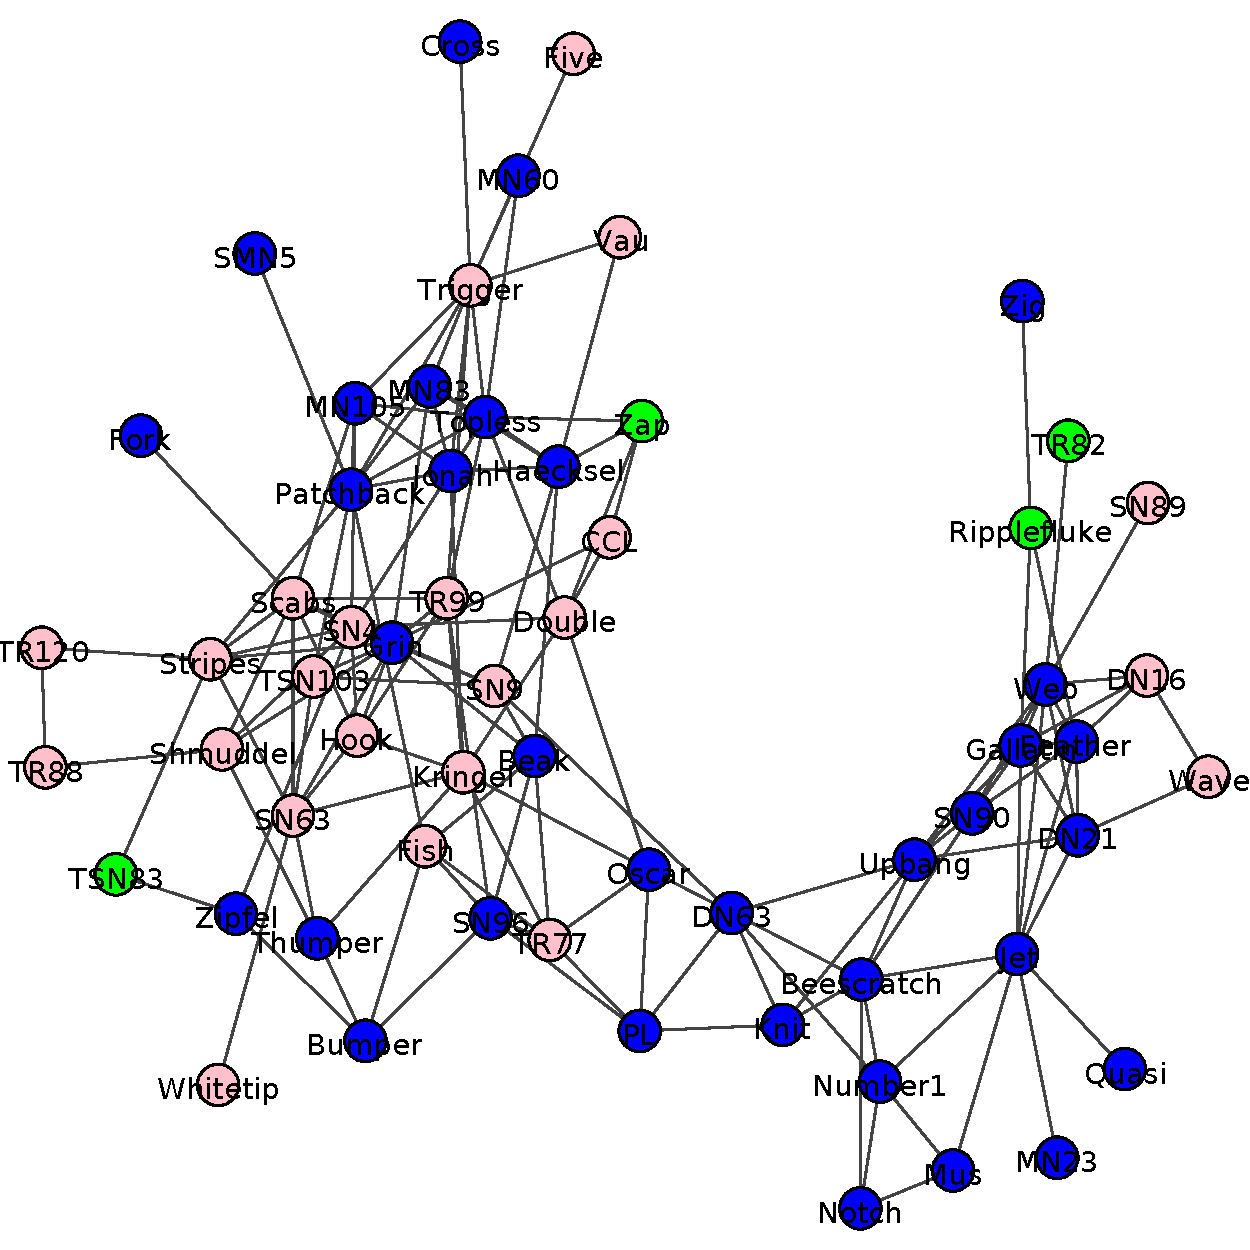
\includegraphics[scale = 0.28]{figuras/Parte_c0-eps-converted-to.pdf} 
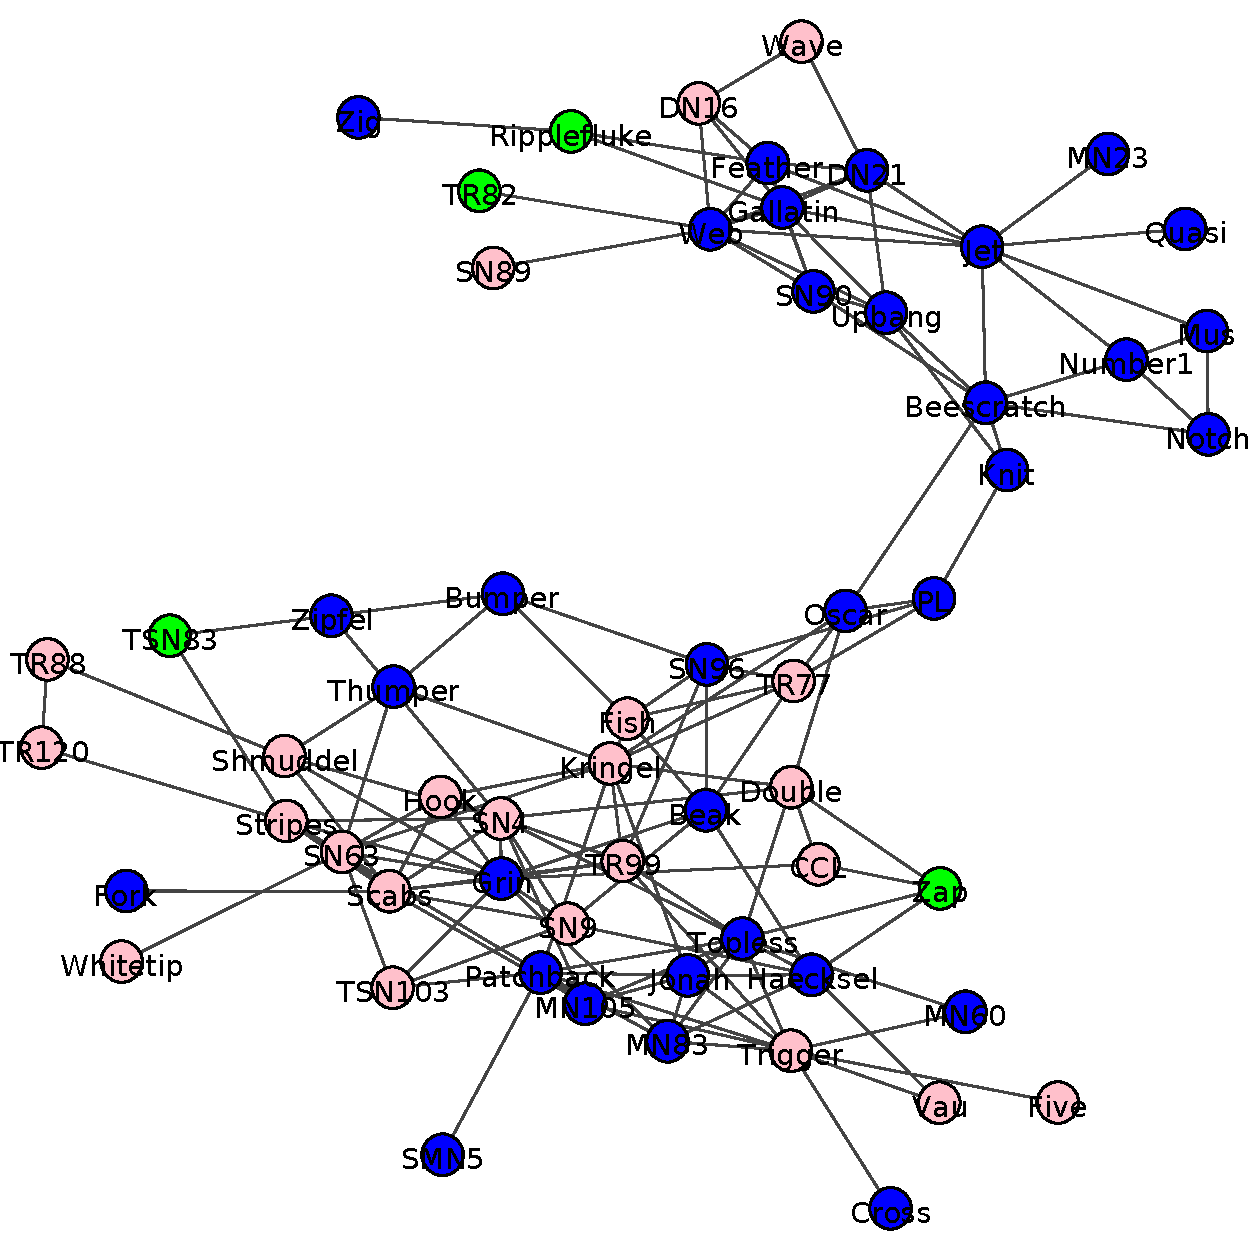
\includegraphics[scale = 0.28]{figuras/Parte_c1-eps-converted-to.pdf} \\
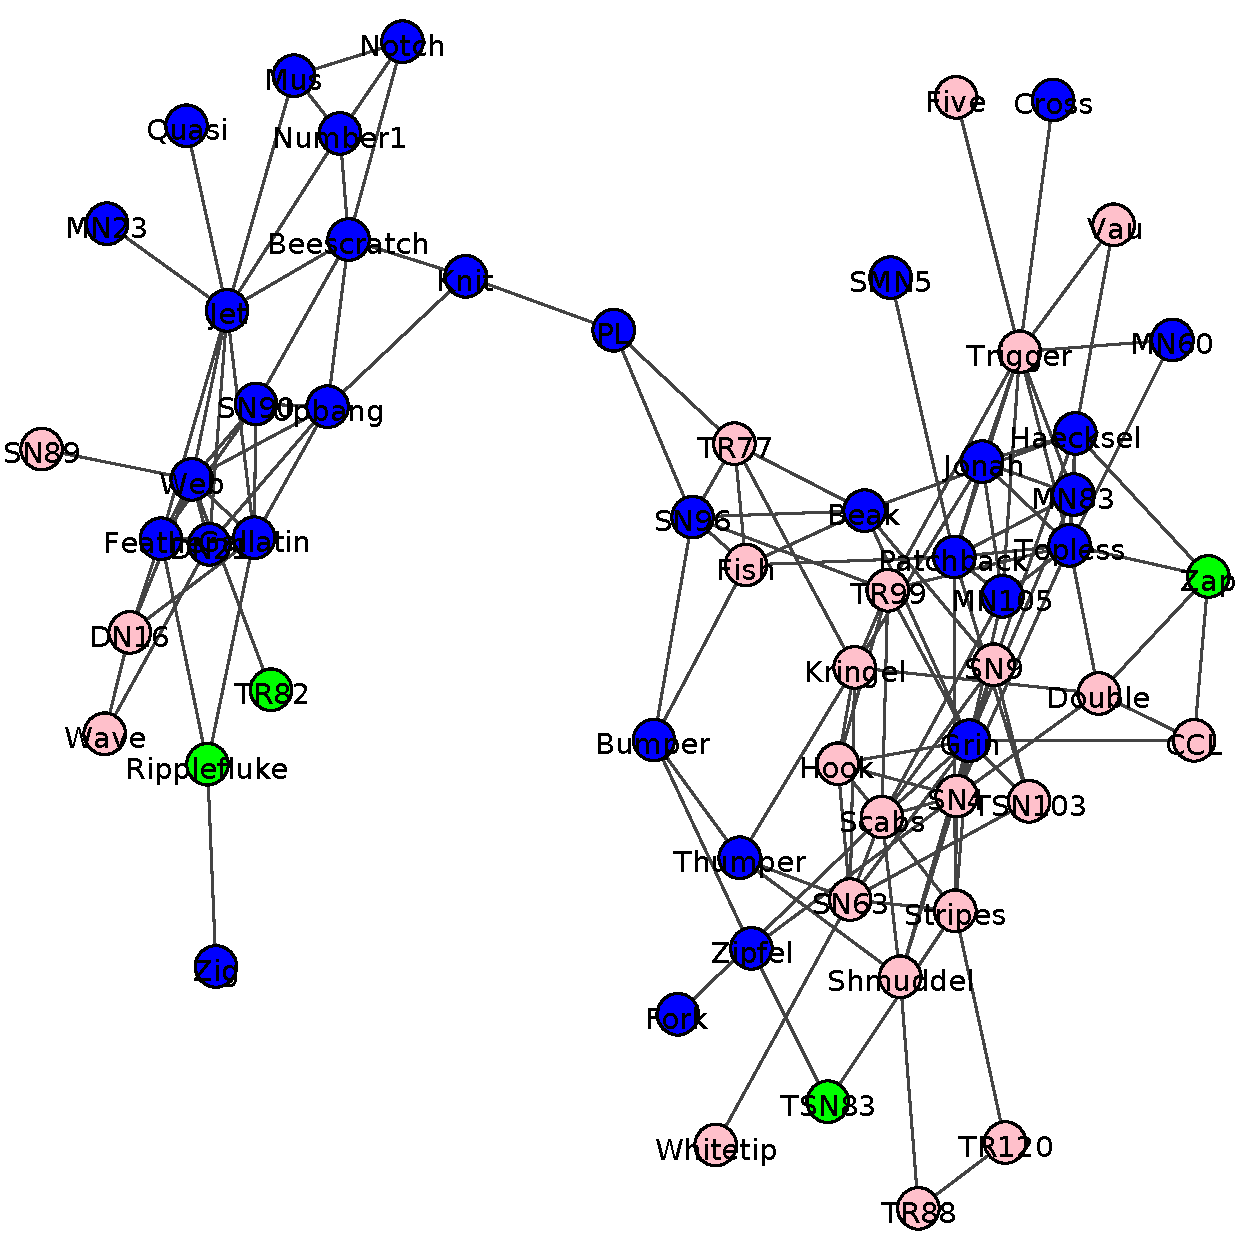
\includegraphics[scale = 0.28]{figuras/Parte_c2-eps-converted-to.pdf} 
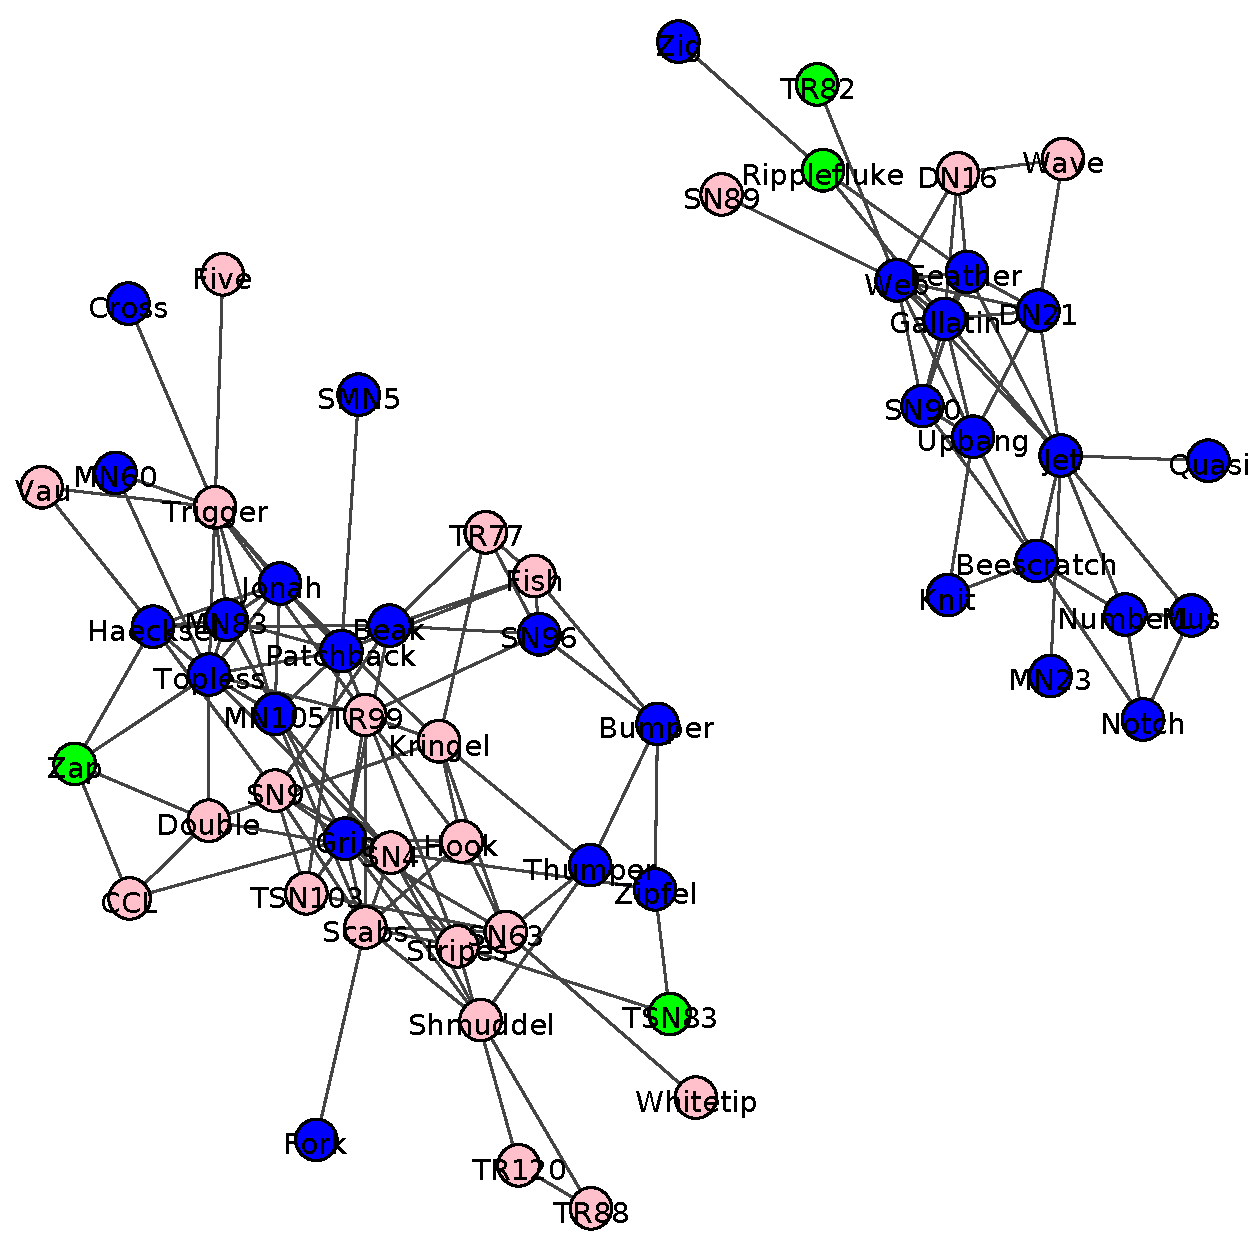
\includegraphics[scale = 0.28]{figuras/Parte_c3-eps-converted-to.pdf} 
\caption{Layout de la red al remover el nodo con mayor betweenness: remoción de izquierda a derecha, y de arriba hacia abajo. Con solo remover 4 nodos, la red se descompone en dos subgrafos de tamaño comparable.}
\label{fig:Betweenness}
\end{figure}

\begin{figure}
\centering
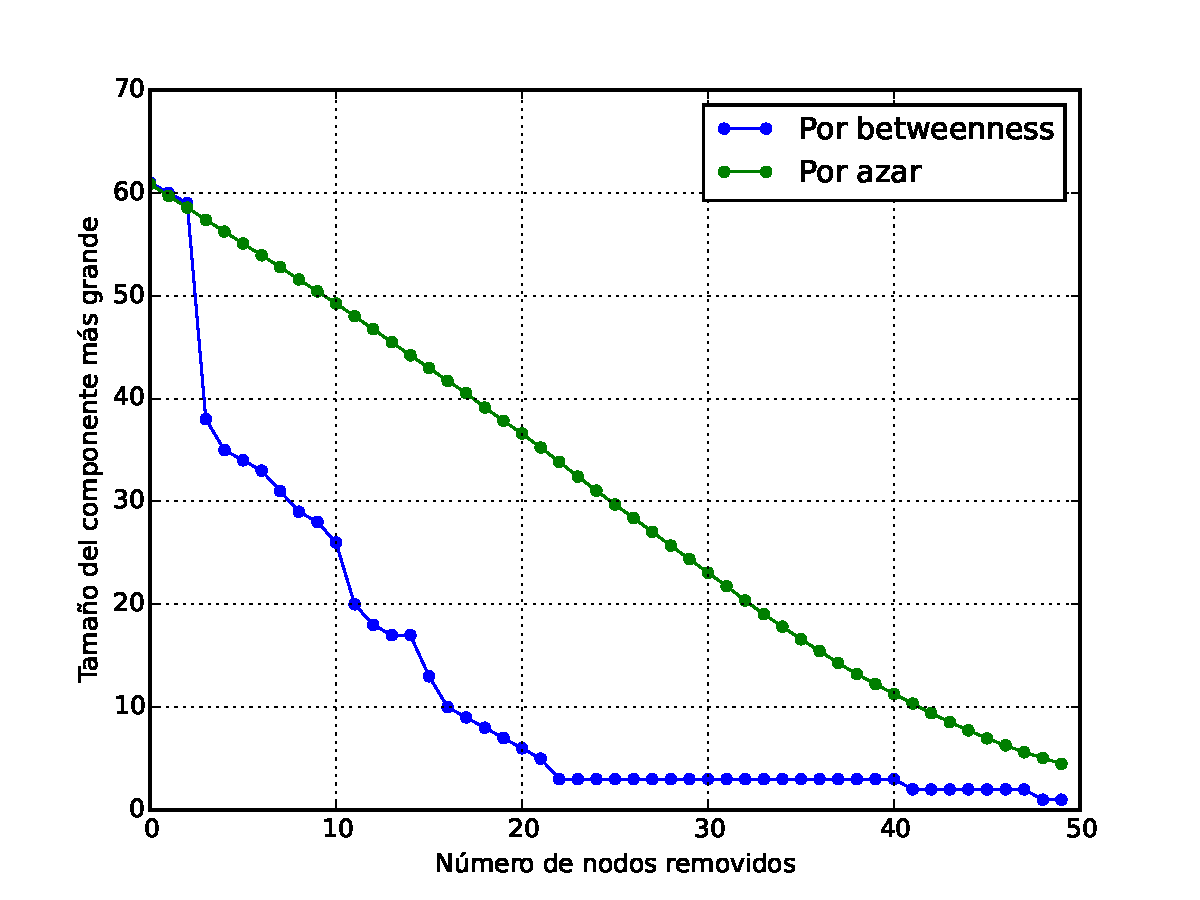
\includegraphics[scale = 0.60]{figuras/Nodos_removidos-eps-converted-to.pdf} 
\caption{Tamaño del componente más grande a medida que se remueven nodos según betweenness, o al azar, respectivamente. Observar la caída abrupta al remover 4 nodos de mayor betweenness. La curva correspondiente a la forma azarosa es un promedio de 1000 configuraciones.}
\label{fig:Comparacion}
\end{figure}
